\documentclass[main.tex]{subfiles}
\begin{document}
	
	There are two ways to utilize the Haskell-Tools framework. The first one is the command line interface, and the second one is the editor integration in Atom. Both interfaces provide more or less the same functionalities. They can be used to load our projects and perform refactorings on the source code. We will discuss both options in the following sections.
	
	\section{Command line interface}
	
	There are two types of refactorings provided by Haskell-Tools: module level refactorings and project-wide refactorings. Also, they can be further divided into two categories based on whether they need a code segment to be selected in order to execute them. For example, renaming a function requires the name of the function to be selected, but organizing imports or extension in a module or a project does not require any selection. If we want to quickly perform an "organizing" refactoring before our daily commit, then the command line interface might be more convenient than browsing through menus in the editor.
	
	We eliminate all unused extensions from our whole project with a single line of command.
	
	%TODO: unescape dollar sign
	\begin{bash}
		\$ stack exec ht-refact -- DIR -e ProjectOrganizeExtensions
	\end{bash}
	
	Generally, any command can be written in place of \pilcode{ProjectOrganizeExtensions}. Also the \pilcode{DIR} argument is the directory of our project.
	
	We can also start an interactive refactoring session using the same interface.
	
	%TODO: unescape dollar sign
	\begin{bash}
		\$ stack exec ht-refact -- DIR
	\end{bash}
	
	During the interactive session, we can issue any number of commands, but our project will be reloaded after every single refactoring. Using the interactive session of the command line interface, we can eliminate the unused extensions from a single with the command below.
	
	\begin{bash}
		ht-refact> OrganizeExtensions MODULE
	\end{bash}
	
	The project-wide refactoring is available during the interactive session as well.
	
	\begin{bash}
		ht-refact> ProjectOrganizeExtensions
	\end{bash}
	
	When we are done refactoring our project, we can simply exit the session.
	
	\begin{bash}
		ht-refact> Exit
	\end{bash}
	
	\section{Atom editor}
	
	If we would like to perform more intricate code transformations, then the Atom editor integration is recommended. First we need to start the Haskell-Tools server.
	
	\begin{figure}[H]
		\hspace{-1cm}
		\centering
		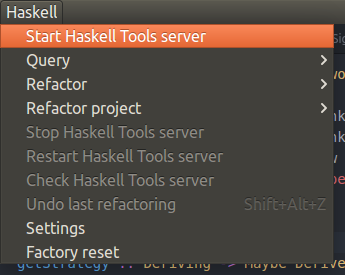
\includegraphics[scale=0.5]{menu_start_server}
		\caption{Starting Haskell-Tools}
		\label{fig:menu_start_server}
	\end{figure}
	
	From now on, the server will be listening for commands. The next step is to add our project to Haskell-Tools. It is important to note, that we should add the folder with the \pilcode{.cabal} file in it. Also, only a single project can be added at a time. The following command will load the modules in our project, and allow us to refactor our source code.
	
	\begin{figure}[H]
		\hspace{-1cm}
		\centering
		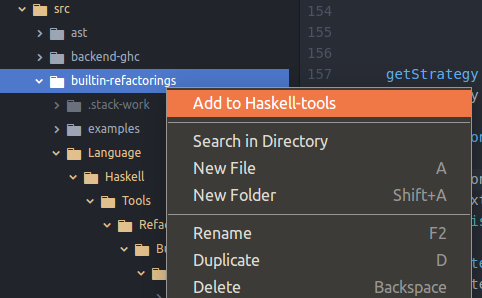
\includegraphics[scale=0.5]{add_project}
		\caption{Adding a project to Haskell-Tools}
		\label{fig:add_project}
	\end{figure}
	
	Using the graphical interface of the editor, we can not only perform refactorings, but so called \emph{queries} as well. Currently, Haskell-Tools only supports a single query which highlights all the language elements in our module that require at least one extension. This quesry option can be found under \pilcode{Haskell > Query}.
	
	\begin{figure}[H]
		\hspace{-1cm}
		\centering
		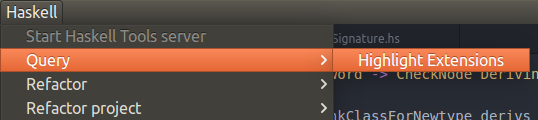
\includegraphics[scale=0.5]{menu_query}
		\caption{Query all language elements requiring certain extensions}
		\label{fig:menu_query}
	\end{figure}
	
	After pressing the button, the editor will underline certain pieces of code requiring language extensions. Hovering over these code segments, a tooltip will appear specifying the required extensions. Besides the extensions, the tooltip also contains information about certainty level associated with the extension(s) which specifies how much confidence we have in the determined extension(s). For example, the \pilcode{Hint} certainty level in the figure below indicates that the language element might not require the determined extension, however, even a subtle code modification can result in the language element actually requiring the extension. So the user should pay close attention to it.
	
	\begin{figure}[H]
		\hspace{-1cm}
		\centering
		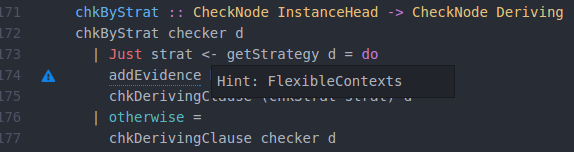
\includegraphics[scale=0.5]{highlight_extensions}
		\caption{Highlighting language elements requiring certain extensions}
		\label{fig:highlight_extensions}
	\end{figure}
	
	\newpage
	
	The graphical interface also supports the features presented in the previous section. The module level extension elimination refactoring can be found under \pilcode{Haskell > Refactor > Organize Extensions}.
	
	\begin{figure}[H]
		\hspace{-1cm}
		\centering
		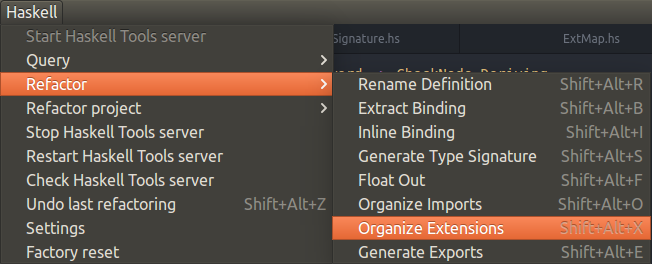
\includegraphics[scale=0.5]{menu_refactor_module}
		\caption{Removing all unnecessary extensions from a module}
		\label{fig:menu_refactor_module}
	\end{figure}
	
	The project level counterpart is located under \pilcode{Haskell > Refactor project > Oranize Extensions}.
	
	\begin{figure}[H]
		\hspace{-1cm}
		\centering
		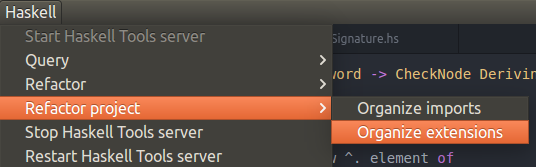
\includegraphics[scale=0.5]{menu_refactor_project}
		\caption{Removing all unnecessary extensions from a project}
		\label{fig:menu_refactor_project}
	\end{figure}
	
	When we are finished with our refactorings, we can stop the server in the same menu. It is advised to close the server after finishing our work with it, since all the modules will be kept in memory as long as the server is running.
	
	\begin{figure}[H]
		\hspace{-1cm}
		\centering
		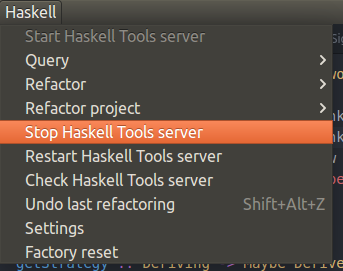
\includegraphics[scale=0.5]{menu_stop_server}
		\caption{Stopping Haskell-Tools}
		\label{fig:menu_stop_server}
	\end{figure}
	
\end{document}